\chapter{第一个人工智能项目（钟咏涛、郑浩男）}

在本章中，我们将深入探讨为什么Python是启动全新且初学者导向的人工智能（AI）项目的理想选择。我们将介绍Python丰富的生态系统，涵盖从底层数据处理到高层模型构建和调优，再到后期部署管理的各个方面。每一层都有适合初学者使用的工具，简化了操作步骤，使新手也能轻松上手。通过具体的应用场景和实例，读者不仅能学到理论知识，还能获得宝贵的实践经验，为未来的项目开发打下坚实的基础。

总之，这一章不仅让读者了解到Python为何重要，还为后续的具体优势和应用场景做好了铺垫。希望你能带着这份信心，勇敢地迈出第一步，探索这个充满无限可能的世界。通过这些内容，我们期待为你提供一个全面而亲切的指南，帮助你在AI编程的道路上越走越远。

\section{人工智能的编程语言Python}

% 在这个AI技术越来越普及的时代，选对编程语言就像是给项目找对了方向，对于新手来说尤其重要。而Python这门语言，就像一位贴心的老朋友，被广泛推荐为开启人工智能之旅的理想选择。它有着简单直白的语法，学起来轻松，用起来顺手，但又不失强大功能，能从研究阶段一路支持到实际应用部署，简直就是一把全能钥匙。Python的历史可以追溯到1991年，由Guido van Rossum发布，它的设计理念就是让代码读起来像日常对话一样自然。随着时间推移，Python逐渐成长为一个多才多艺的语言，适应各种需求。到了互联网和大数据时代，Python在数据科学和机器学习领域开始大放异彩。它先是通过NumPy、SciPy等库为数值计算和数据分析提供了坚实的基础，后来又随着机器学习和深度学习的发展，加入了scikit-learn、TensorFlow和PyTorch这些强大的工具，简化了AI模型的构建，降低了进入这个领域的门槛。

% 不仅是初创公司，就连Google、Facebook和微软这样的科技巨头也都在用Python来推动他们的AI研究和产品开发。Python之所以这么受欢迎，很大程度上是因为背后有一个庞大而又友好的社区。这个社区里的人们乐于分享知识和技术经验，不断贡献开源项目，形成了一个丰富多彩的生态系统。无论是在Stack Overflow还是GitHub上，你都可以找到无数关于Python的帮助和支持，这对于新入门的开发者来说简直是如获至宝。总之，选择Python不仅是因为它好用，更因为它背后的社区让你感受到家一般的温暖和支持。

% 尽管我们已经对Python在AI领域的价值进行了较为全面的介绍，但这仅仅是冰山一角。随着技术的不断进步，Python及其相关工具将继续推动AI的发展边界。因此，我们强烈鼓励读者继续深入探索Python在这一激动人心领域的更多可能性。接下来的小节将带领您深入了解Python在不同AI任务中的具体应用案例，例如如何使用Python构建高效的自然语言处理系统、如何利用计算机视觉技术实现图像识别，以及如何通过强化学习创建智能决策算法。此外，我们还将探讨如何运用Python搭建从研究到生产的完整工作流，包括模型训练、验证、部署及运维等各个环节的最佳实践。

在这个AI技术越来越普及的时代，选对编程语言就像是给项目找对了方向，对于新手来说尤其重要。而Python这门语言，被广泛推荐为开启人工智能之旅的理想选择。之所以Python能够有这样的地位，主要归功于其简洁易读的语法、强大的功能以及丰富的工具库。此外，Python自1991年发布以来，以直观的设计理念迅速成长为适应多种需求的全能型语言。特别是在数据科学和机器学习领域，Python凭借NumPy、SciPy、scikit-learn、TensorFlow和PyTorch等库简化了数值计算、数据分析及AI模型构建的过程。

Python的强大不仅体现在技术层面，还在于它背后有一个庞大且活跃的社区。这个社区不断贡献开源项目和技术支持，形成了一个丰富多彩的生态系统，对于新手开发者尤其友好。无论是大型科技公司还是初创企业，Python都是推动AI研究和产品开发的重要工具。此外，选择Python进行AI开发，不仅能享受到高效便捷的编程体验，还能获得来自社区的广泛支持。随着技术的进步，Python及其生态将继续扩展AI的应用边界，为开发者提供无限可能。在下面的章节中将深入探讨Python在具体人工智能任务中的应用案例及其在工作流各环节的最佳实践。

\subsection{Python简介与特点}

\subsubsection{1. 量身定制的编程语言}

Python就像是一种能让你和电脑对话的语言，而且这种对话是用一种非常接近我们日常交流的方式进行的。它的设计初衷就是要让代码看起来尽可能像人类自然的语言，所以你不会看到那些让人眼花缭乱的符号和复杂的语法规则。这就是为什么Python被称作“优雅”的编程语言——因为它不仅简洁明了，还能用最少的代码完成很多事情。比如说，如果你想要打印一句话，其他编程语言可能会要求你写好几行代码，而Python只需要一行,如图\ref{fig:Python代码}所示：

\begin{figure}[H]
    \centering
    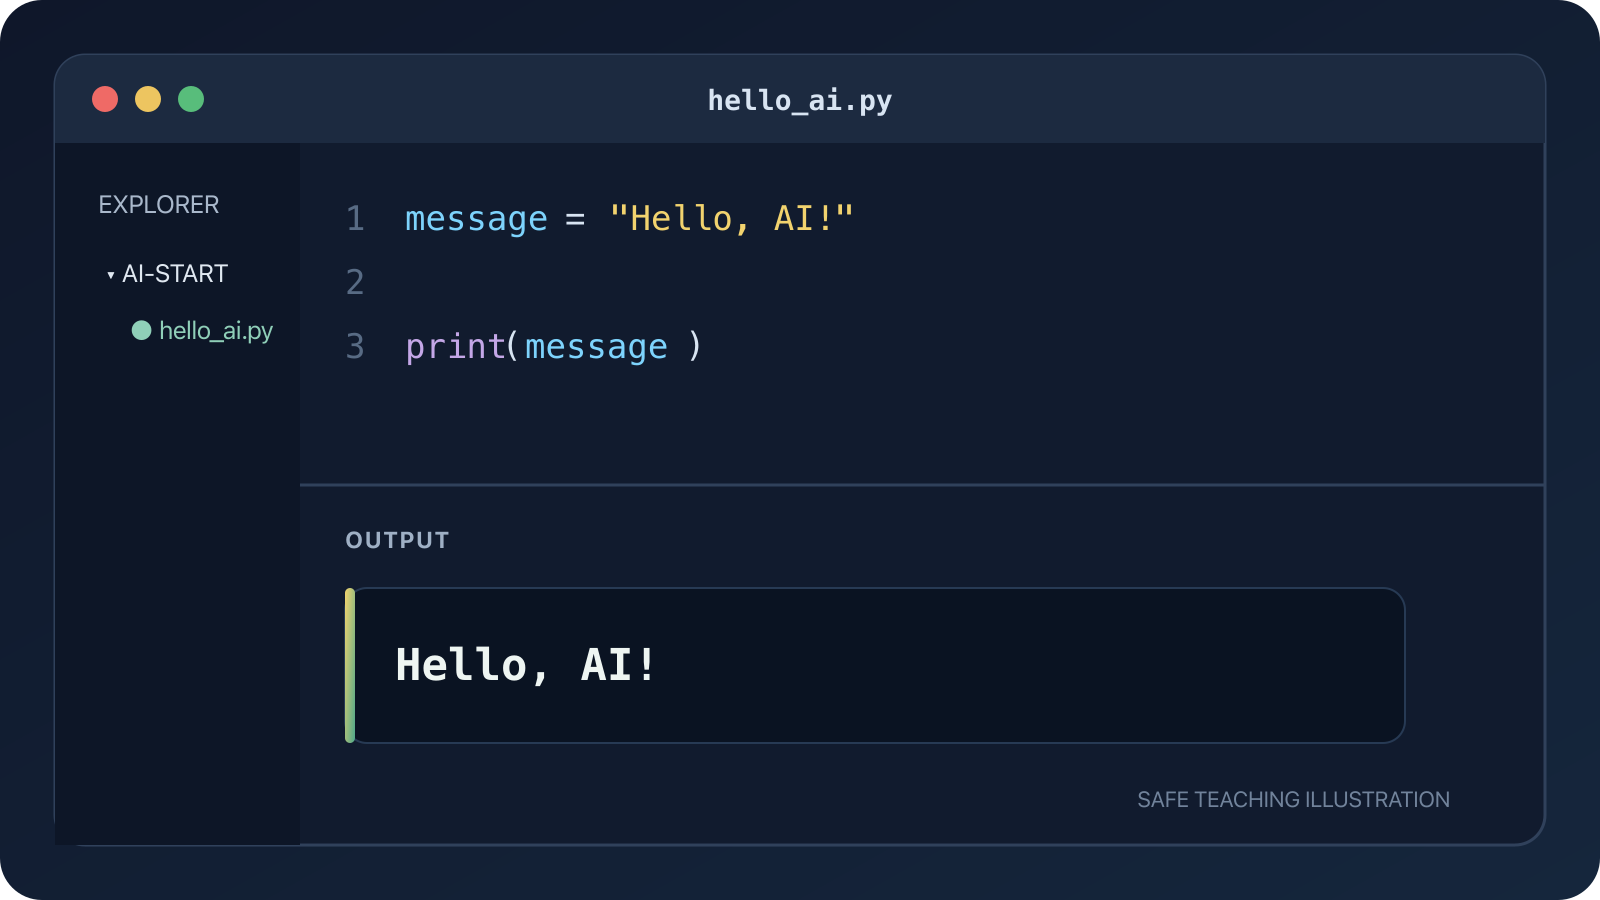
\includegraphics[width=0.8\linewidth]{image/6/python-code-safe.png}
    \caption{Python打印一句话}
    \label{fig:Python代码}
\end{figure}

Python就像是为新手量身定做的，它有着清晰的一致性和逻辑结构，这意味着一旦你理解了一个概念，就可以很容易地将这个知识应用到其他地方。比如，在Python中定义一个函数，你会发现它的格式和其他很多操作都很相似，这使得学习新东西变得更加容易。想象一下，如果把编程比作做饭，那么Python就像是有一本超级详细的食谱书，每一步都解释得清清楚楚，甚至还有图解。这样一来，即使是第一次进厨房的新手，也能按照指示做出一道美味佳肴。对于编程新手来说，Python就是这样一本“食谱”，它让你能够快速上手，并且很快就能写出有用的程序来。

Python还有一个特别酷的地方，那就是它不仅仅局限于一种编程方式。你可以选择你喜欢或者最适合解决问题的方式来编写代码。有时候你可能想用面向对象编程（OOP），这时候Python允许你创建类和对象，就像在现实生活中给事物分类一样；但如果你觉得过程化编程更符合你的思路，Python也完全支持，你可以直接写一个个小函数来做事情；甚至如果你想尝试函数式编程，Python也不会让你失望，它同样提供了相应的工具和支持。这就像是给你一把万能钥匙，不管你想打开哪种类型的锁，Python都能帮你做到。无论你是喜欢按部就班地解决问题，还是倾向于更加灵活多变的方法，Python都可以满足你的需求。这样，你不仅可以根据自己的喜好来选择最舒服的方式编程，还可以根据具体问题的特点挑选最合适的方法，真正做到游刃有余。


\subsubsection{2. 学习曲线与开发效率}

想象一下，你有一个绝妙的想法，想要立刻看到它变成现实。Python就像是你的魔法棒，能让你快速地把脑海里的想法转化为实际的代码和功能。特别是在人工智能（AI）领域，很多时候我们需要不停地尝试新思路，调整算法，看看它们的效果如何。这个时候，Python的速度优势就显得特别重要了。比如说，你想做一个简单的AI模型来识别图片中的动物。用Python，你可以很快搭建出一个基础框架，导入必要的库，然后在短时间内让程序跑起来。这不仅节省了时间，还让你可以更快地测试不同的想法，找到最适合的解决方案。这种快速迭代的能力，在AI项目中简直是无价之宝，因为它帮助我们更快地从失败中学习，不断改进。

说到编程，它有时候就像解谜游戏，而调试就像是寻找隐藏的宝藏。Python的动态类型系统和交互式shell（比如IPython或Jupyter Notebook），就像是给你配备了高级的寻宝地图和工具。当你在编写代码时遇到问题，这些工具可以帮助你更快地发现错误，并且马上进行修复。例如，如果你不确定某一行代码是否正确，可以在交互式shell里直接运行这段代码，看看它的输出是不是符合预期。如果不对，你可以立即调整代码并再次测试，整个过程非常流畅。而且因为Python是动态类型的，你不需要提前声明变量类型，这使得编写和修改代码更加灵活快捷。

Python简直就是一块万能积木。它不仅可以自己玩得很好，还能和其他语言和技术完美合作。在人工智能项目中，我们经常需要结合多种技术，比如使用C++编写高性能计算模块，或者集成Java的企业级应用。Python就像一个超级中介，能轻松地把这些不同部分连接在一起，让它们协同工作。举个例子，如果你正在开发一个人脸识别系统，可能需要用深度学习框架如TensorFlow或PyTorch来处理图像数据，同时还需要调用一些硬件接口或Web API来获取实时信息。Python可以通过各种库和工具轻松实现这一点，为开发者提供了极大的便利。这就像是在一个团队里，Python担任着协调者的角色，确保每个成员都能发挥最佳状态，共同完成复杂的任务。

\subsubsection{3. 社区与资源背景}

当你选择Python作为你的编程语言时，就像是加入了一个大家庭。这个大家庭遍布全球，有成千上万的开发者和爱好者。无论你是在白天遇到问题，还是深夜突然有了新想法，几乎总能找到同行的帮助或指导。想象一下，当你在编写代码时遇到了难题，只需要在社区论坛上发帖，很快就会有人回应你，给出建议和支持。这种感觉就像有一个随时待命的朋友圈，只要你需要帮助，他们就在那里，如图\ref{fig:Python社区}所示。

\begin{figure}[H]
    \centering
    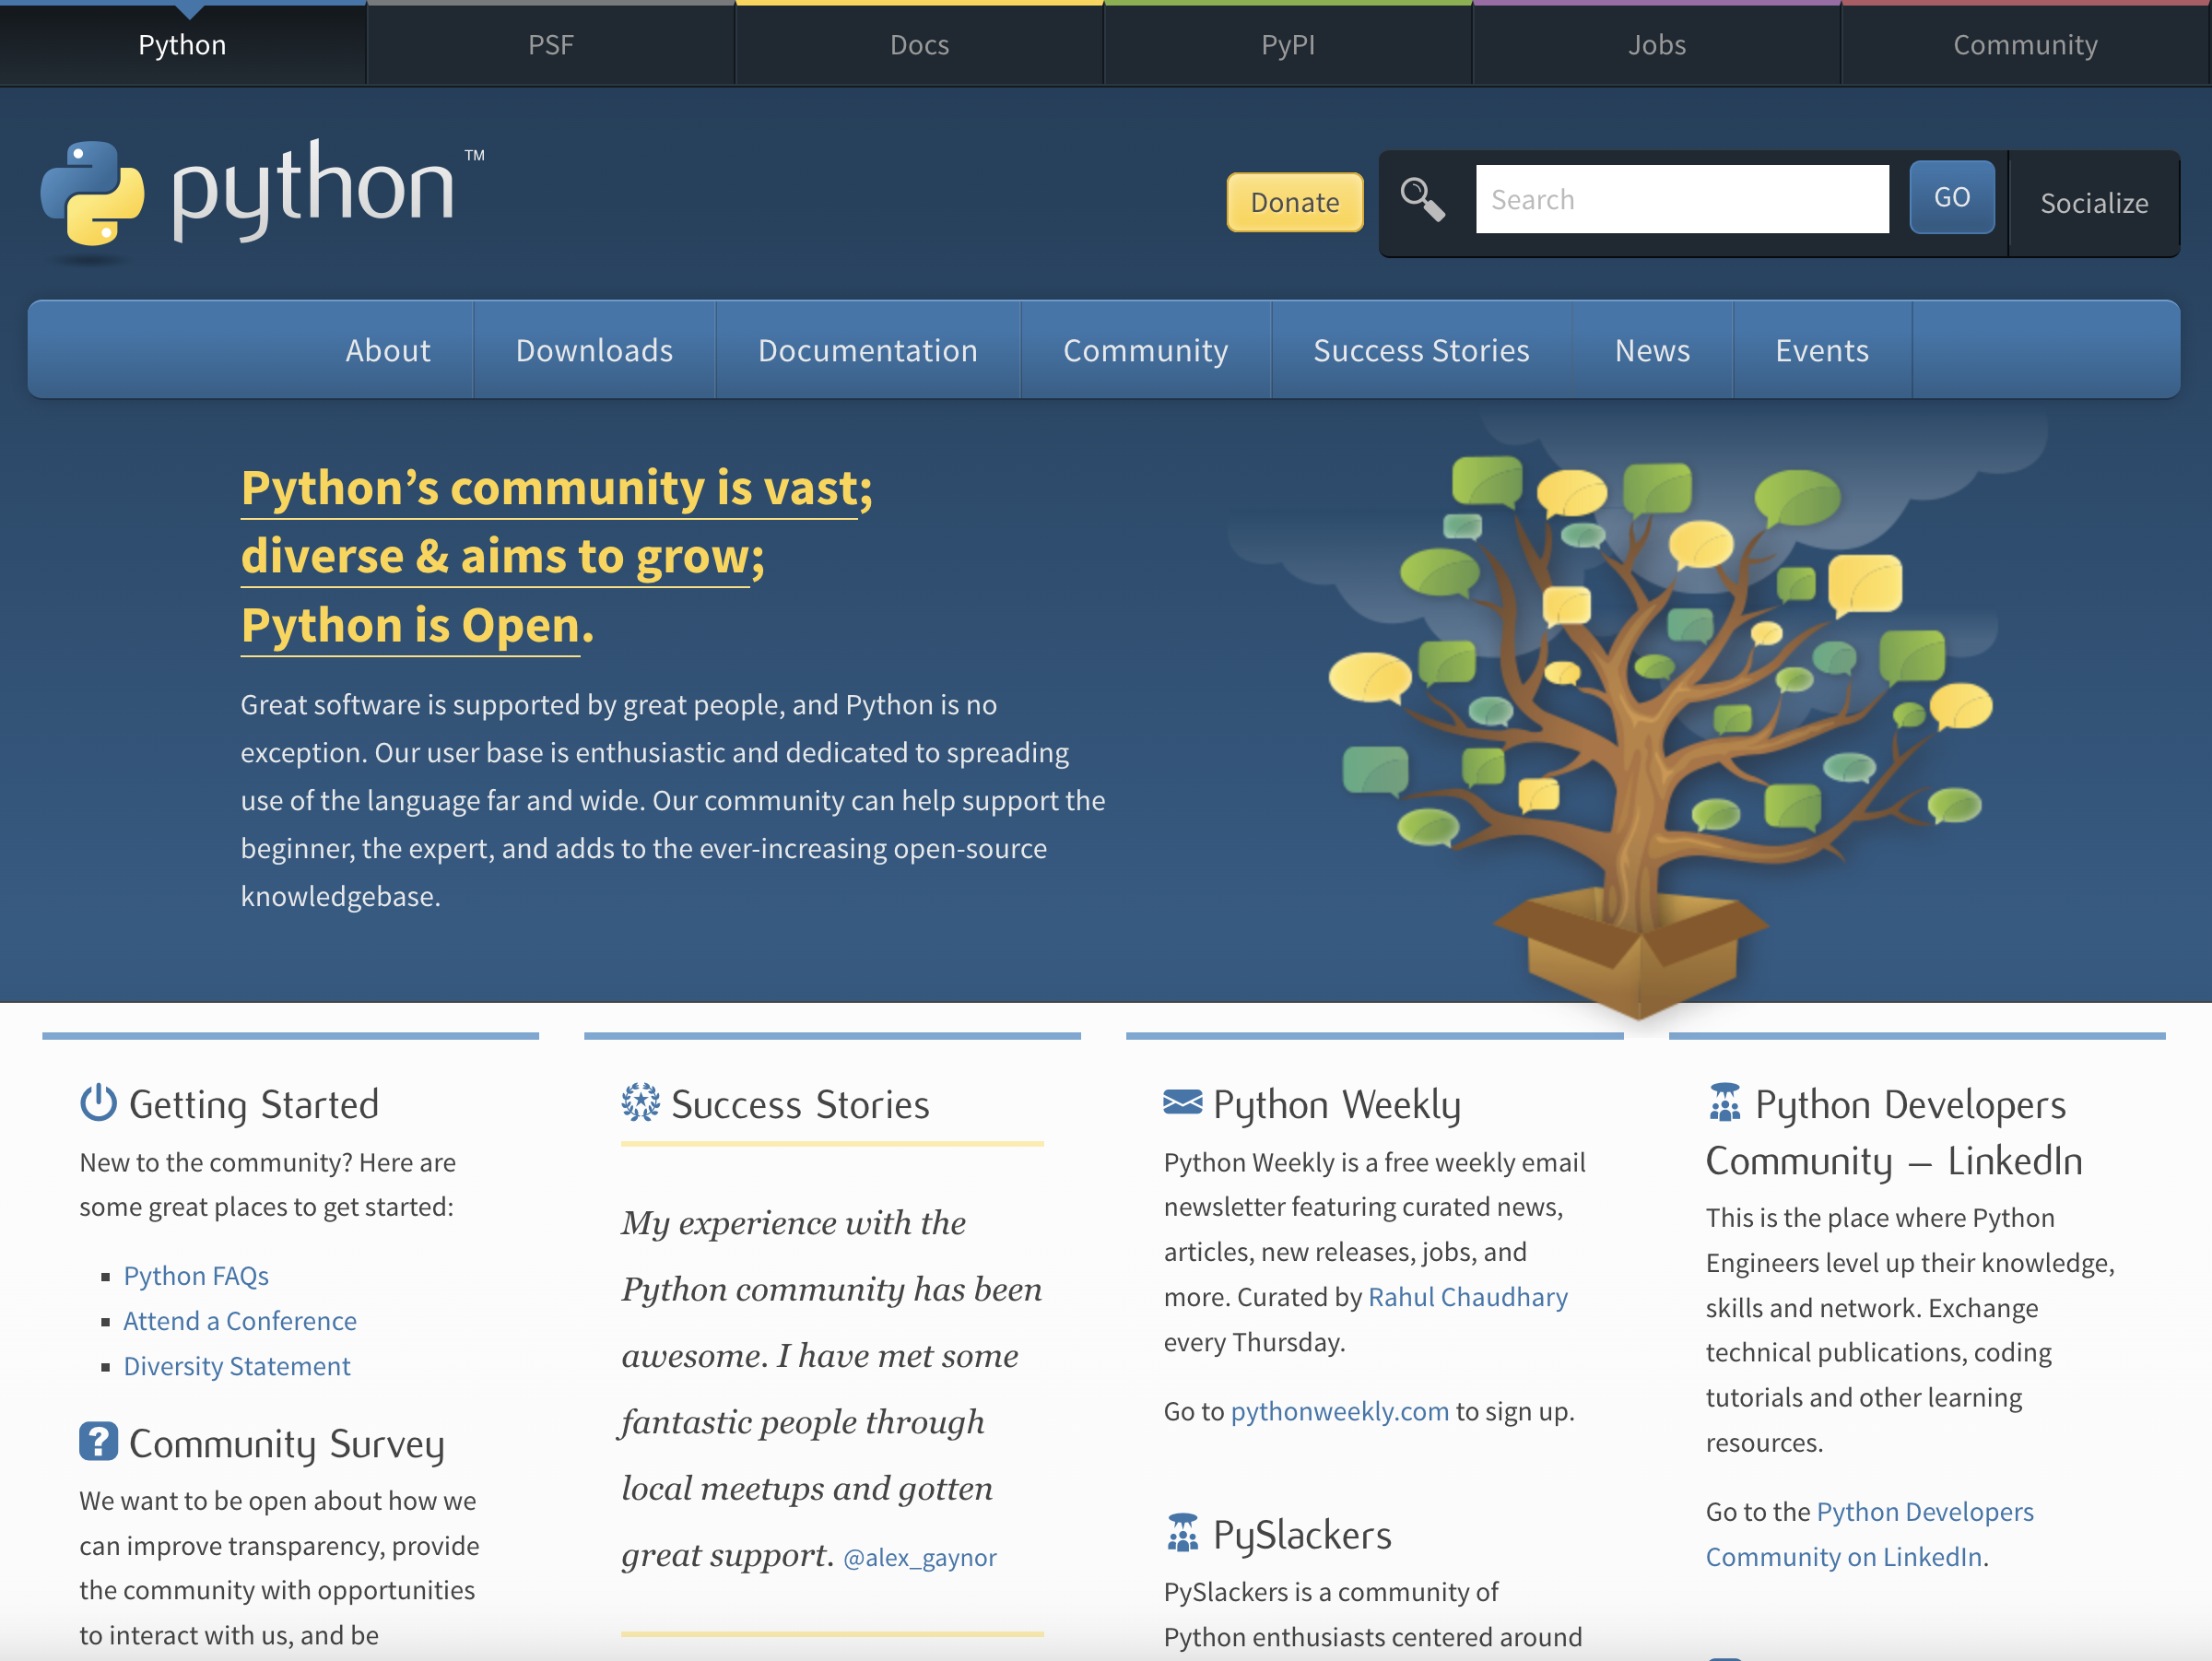
\includegraphics[width=0.8\linewidth]{image/6/Python社区.png}
    \caption{Python社区}
    \label{fig:Python社区}
\end{figure}

Python社区非常包容和友好。新手不用担心问“蠢问题”，因为大家都曾经是初学者，都明白那种无助的感觉。在这里，每个人都可以分享自己的经验、技巧，甚至是一些小窍门，帮助他人更快地成长。这不仅让学习变得轻松愉快，还让你感受到一种归属感和温暖。

通过这样的Python社区，能够让学习Python并不孤单，这一点非常重要。无论你是喜欢看书自学，还是更倾向于看视频教程，又或者是想通过实践来提高技能，Python都能满足你的需求。网络上有大量的教程、文档、在线课程和论坛，它们就像是为不同口味的人准备的各种美食，总有一款适合你。比如，有些人喜欢跟着详细的步骤一步步来，网上有很多结构化的教程可以带你从零开始；如果你是个视觉学习者，那么有许多生动的视频教程等着你去探索；而那些喜欢自己动手解决问题的人，则可以通过参与各种项目和挑战，在实践中学习。无论你喜欢哪种方式，Python社区都会为你提供足够的资源和支持，让你的学习之路充满乐趣而不感到孤单。

所以Python不仅仅是一个编程语言，它更像是一个不断进化的生态系统。这个生态系统的各个部分——库、框架、工具等等——都在不停地更新和发展。这意味着，随着技术的进步，Python也在与时俱进，始终保持在科技前沿。对于从事人工智能研究的人来说，这一点尤为重要。例如，新的机器学习算法出来了，很快就会有相应的Python库出现，让你能够快速应用这些新技术。如果某个领域出现了突破性的进展，Python社区也会迅速反应，开发出相关的工具和资源。这就像是在一个不断成长的花园里，每一种植物（库和框架）都在茁壮成长，为整个花园（Python生态系统）增添了色彩和活力。选择Python，你就等于选择了持续进步的机会。无论是现在流行的深度学习、数据分析，还是未来的新兴技术，Python都能为你提供最先进、最适合的工具。这样，你不仅可以紧跟时代的步伐，还能在这个过程中不断成长和创新。


\subsection{Python在人工智能中的作用}

\subsubsection{1. 连接研究与应用的过程}
    
想象一下，Python就像是一个超级翻译官，它能够把复杂的学术理论转化为实际可以用的产品。无论是研究人员在实验室里探索新想法，还是企业想把这些创新技术变成真正的产品推向市场，Python都能起到关键的桥梁作用。比如说，研究人员可能会发明一种新的机器学习算法，这个算法听起来可能非常高深莫测，但通过Python，他们可以快速编写代码来验证这个算法是否真的有效。Python简单易懂的语法和丰富的库，使得即使是复杂的数学公式也能轻松实现。这样一来，研究人员不仅能够证明他们的想法是对的，还能展示出实际的效果。并且对于企业来说，Python同样是一个得力助手。当他们看到某个新技术有潜力时，就可以用Python迅速开发一个原型，看看这个技术能不能真正解决问题。如果效果不错，Python还能直接用于最终产品的开发，而不需要重新用其他语言重写。这就大大节省了时间和成本，让创新技术更快地落地生根。

现在，让我们聊聊Python如何帮助AI技术从实验室走向生产环境。你可能觉得这听起来像是个大工程，但实际上，Python让它变得非常简单。假设你在实验室里开发了一个很棒的AI模型，它可以识别图片中的物体。接下来，你想把这个模型放到一个真实的应用中，比如一个手机APP，让人们可以通过拍照识别植物或动物。这时候，Python的优势就显现出来了。因为它不仅仅是一种适合实验的语言，还非常适合部署到实际环境中。你可以使用Python编写的所有代码、工具和库，直接将你的模型集成到最终产品中，甚至可以直接部署到云端。这种灵活性和效率，使得Python成为推动技术创新和商业价值转化的关键力量。企业不再需要花费大量时间等待技术从实验室走出来，而是可以在短时间内就把最新的研究成果应用到实际产品中，为用户提供更好的服务。Python就像是一个加速器，帮助我们更快地把好点子变成现实，让更多人受益于这些创新技术。

通过这样的过程，Python不仅连接了学术研究和产业实践，还在两者之间架起了一座坚实的桥梁，确保每一个好的想法都能顺利地从实验室走进我们的日常生活。这就是为什么Python在全球范围内如此受欢迎，尤其是在人工智能领域——它让科技变得更加贴近生活，也让创新变得更加容易实现。

\subsubsection{2. 贯穿AI项目全流程}

刚才我们聊了Python如何作为桥梁，把学术研究和产业实践连接起来，并且让新技术能够快速从实验室走向市场。接下来，让我们看看Python在整个AI项目中是如何一步步帮助我们完成任务的，从最初的准备到最后的应用，每一步都不简单。

\begin{itemize}
\item \textbf{数据准备}

在开始任何AI项目之前，数据就像是建造房子的砖块，没有好的砖块，再漂亮的设计也无济于事。Python在这里就扮演了“砖瓦匠”的角色，它能帮你收集、清洗和预处理数据，确保这些“砖块”质量过硬，为后续的工作打下坚实的基础。想象一下，你有一个杂乱无章的数据集，里面可能有缺失值、错误信息，甚至格式不一致。用Python，你可以轻松地清理这些数据，剔除不需要的部分，填补缺失的地方，让数据变得整洁有序。Python的各种库，比如Pandas和NumPy，就像是你的得力助手，让你的数据准备工作变得更加高效和准确。


\item \textbf{模型训练}

当你有了干净的数据后，下一步就是选择合适的算法来解决问题。这里Python就像一个大超市，里面有各种各样的工具和方法供你挑选。你可以尝试不同的机器学习或深度学习算法，看看哪个最适合你的问题。Python的灵活性使得这个过程非常方便，你可以迅速编写代码来测试不同的模型，比较它们的效果，找到最合适的解决方案。比如说，你想做一个预测销售量的模型，可以用Python试试线性回归、决策树、随机森林等各种算法，看看哪种方法预测得最准。这种灵活多变的能力，让开发者可以在短时间内探索多种可能性，找到最优解。

\item \textbf{参数调整}

一旦选定了算法并训练好模型，接下来就要确保这个模型是可靠的。这就像是给新造的房子做安全检查，Python在这里帮了大忙。通过Python，你可以对模型进行验证和优化，确保它的预测结果既准确又稳定。比如说，你可以使用交叉验证等技术来评估模型的表现，看看它在不同数据上的表现是否一致。如果发现某些地方不够理想，还可以进一步调整参数，优化模型性能。Python提供的丰富工具和库，如Scikit-learn，使这个过程变得直观而有效。

\item \textbf{结果展示}

当你有了一个好的模型之后，怎么把这个复杂的结果展示给别人看呢？这时候Python就像是一个出色的讲解员，它可以帮助你将复杂的分析结果以直观的方式呈现出来。无论是生成图表、制作报告，还是创建交互式仪表盘，Python都能胜任。例如，你可以用Matplotlib或Seaborn这样的，把模型的预测结果变成漂亮的图表，让非技术人员也能一目了然。或者，如果你需要向管理层汇报，Python还能帮你生成专业的报告，清晰地传达你的发现和建议。最后，当一切准备就绪，模型需要被部署到实际环境中，开始为用户提供服务。Python在这个阶段同样表现出色，它提供了多种工具和框架，确保从开发到上线的顺利过渡。无论你是想把模型部署到云端，还是嵌入到移动应用中，Python都能提供相应的支持，简化这个过程。举个例子，如果你想把识别图片的模型集成到一个手机APP中，Python可以帮助你打包模型，让它能够在移动设备上运行。或者，如果你打算把模型放到云端，Python也可以与云服务无缝对接，让你的模型随时随地为用户服务。
\end{itemize}

通过这样一步一步的流程，Python不仅贯穿了整个AI项目的生命周期，还确保每个环节都能高效、可靠地完成。正是这种全面的支持，让Python成为了AI开发者们不可或缺的伙伴，也让AI技术能够更快、更好地从实验室走进我们的日常生活。

\subsection{常用的Python库与工具}

\subsubsection{1. 生态丰富性与层次性}


Python的生态系统就像是一个精心设计的工具箱，里面装满了各种各样的工具，从最基础的数据处理到最高级的模型部署，每一步都有相应的解决方案。这个工具箱不仅层次分明，而且功能完备，不管你是在哪个阶段，都能找到合适的工具来帮你完成任务。在数据处理阶段，你需要对原始数据进行清洗、转换和预处理。Python提供了丰富的库，让你可以轻松搞定这些工作，确保数据的质量和适用性。接下来，当你进入特征工程时，Python同样有强大的工具可以帮助你提取和选择最有用的特征，为后续的模型训练打下坚实的基础。再往上一层，到了模型构建和调优阶段，Python更是大显身手。你可以利用各种机器学习和深度学习库，快速搭建和训练模型，并通过优化工具不断提升模型的性能。最后，当你准备把模型部署到实际环境中时，Python还能提供一系列工具，确保你的模型能够顺利上线，为用户提供服务。

Python的这种层次分明、功能完整的生态体系，确保了无论你在项目的哪个阶段，都能得到高效的支持。无论是数据准备、模型训练、性能评估，还是最终的产品部署，Python都为你准备好了丰富的工具和库。比如，在数据准备阶段，Python提供的工具不仅强大，还非常友好，即使是初学者也能轻松上手。在模型训练阶段，Python的灵活性让你可以快速尝试不同的算法，找到最适合问题的解决方案。而在性能评估阶段，Python的各种验证和优化工具，能确保你的模型既准确又可靠。最后，在产品部署阶段，Python提供的工具使得整个过程变得更加顺畅，减少了从开发到上线的时间和复杂度。这种全面的支持，就像是有一个经验丰富的导师在旁边指导你，每一步都给你提供最合适的方法和工具。无论你是刚开始接触AI的新手，还是已经有一定经验的开发者，Python都能满足你的需求，帮助你顺利完成每一个环节的工作。

通过这种方式，Python不仅连接了各个开发阶段，还在每个阶段都提供了强有力的支持，确保你能高效、顺利地完成整个AI项目。这正是Python之所以成为AI开发者们首选语言的原因之一——它不仅仅是一个编程语言，更是一个全方位支持你实现梦想的强大伙伴。

\subsubsection{2. 不同阶段的工具特征}

Python为初学者无论是在数据处理、模型训练、性能评估还是结果展示阶段都提供了大量工具，就像是一位贴心的导师，帮助你轻松上手。想象一下，你刚开始接触AI，可能会觉得每个步骤都很复杂，不知道从哪里下手。别担心，Python的生态系统专门为初学者准备了很多简单易用的工具。这些工具简化了各个阶段的操作，让你即使没有太多经验也能顺利进行开发。接下来，我们就来详细看看这些工具是如何帮助你的。

\begin{itemize}

\item \textbf{数据处理}

首先，我们来看看数据处理阶段。你知道吗？数据就像是烹饪的原材料，只有优质的食材才能做出美味的菜肴。Python有很多工具可以帮助你简化数据转换和预处理，使数据准备工作变得更加直观和高效。比如说，Pandas这个库就像是你的厨房助手，它能帮你轻松清洗和整理数据，剔除不需要的部分，填补缺失的数据点。通过简单的几行代码，你就可以把杂乱无章的数据变得整洁有序，为后续的工作打下坚实的基础。

\item \textbf{模型训练}

当你有了干净的数据后，下一步就是训练模型了。这时候，Python就像是一个大超市，里面有各种各样的机器学习和深度学习算法供你挑选。你可以快速调用这些算法接口，尝试不同的模型，找到最适合问题的解决方案。例如，Scikit-learn这个库提供了许多易于使用的算法接口，即使是新手也能快速上手。你可以用它试试线性回归、决策树、随机森林等各种算法，看看哪个最适合你的数据。这种灵活多变的能力，让开发者可以在短时间内探索多种可能性，找到最优解。

\item \textbf{模型优化}

训练好模型后，当然要确保它真的有效。这就像是给新造的房子做安全检查，Python在这里帮了大忙。通过Python，你可以对模型进行验证和优化，确保它的预测结果既准确又稳定。比如，你可以使用交叉验证等技术来评估模型的表现，看看它在不同数据上的表现是否一致。如果发现某些地方不够理想，还可以进一步调整参数，优化模型性能。Python提供的丰富工具和库，如Scikit-learn，使这个过程变得直观而有效。

\item \textbf{可视化工具}

当你有了一个好的模型之后，怎么把这个复杂的结果展示给别人看呢？这时候Python就像是一个出色的讲解员，它可以帮助你将复杂的分析结果以直观的方式呈现出来。无论是生成图表、制作报告，还是创建交互式仪表盘，Python都能胜任。例如，Matplotlib或Seaborn这样的可视化库，可以让你把模型的预测结果变成漂亮的图表，让非技术人员也能一目了然。或者，如果你需要向管理层汇报，Python还能帮你生成专业的报告，清晰地传达你的发现和建议。


\end{itemize}

在本章中，具体介绍了Python在AI项目不同阶段提供的工具，从数据处理到结果展示，每个环节都有适合初学者使用的友好工具。在之后的部分，将通过一系列具体的应用场景和实例组装出一个可运行的项目原型。并帮助初学者发现，有了前文中提到的这些成熟工具，整个构建过程并不复杂。比如，如何用Pandas清洗和整理数据，用Scikit-learn训练模型，再用Matplotlib生成直观的可视化结果。

此外，在接下来的章节还会引导初学者逐步解决问题。更重要的是，你会发现自己能够独立完成复杂的项目，不再害怕面对新的挑战。通过这些实际操作与示例章节，初学者不仅能学到理论知识，还能获得宝贵的实践经验，为未来的项目开发打下坚实的基础。Python具备强大工具和友好的学习环境，足够帮助初学者在AI领域走得更远。无论是深入研究还是应用于实际工作，这些动手实践的经验都将非常宝贵。

\section{平台介绍}
为了帮助读者免去复杂的环境配置，我们开发了一套专为人工智能学习设计的数字平台（\href{https://szjc.ncu.edu.cn/}{https://szjc.ncu.edu.cn/}）。平台仅面向南昌大学及本书官方授权学校的师生开放，具体功能与登录权限以平台实际页面为准。
无论您是否有编程经验，这个平台都能帮助您轻松入门，让您专注于学习和实践人工智能的基础知识和核心技术。

我们的平台不仅支持代码编辑和即时运行，还内置了人工智能相关的工具链和预配置环境，免去了繁琐的环境搭建过程。

以下是平台的核心特点：
\begin{itemize}
    \item \textbf{即开即用的环境}：无需手动配置任何依赖，平台已预装了常用的深度学习框架（TensorFlow），以及支持数据处理和可视化的工具库（如 Pandas 和 Matplotlib）。
    \item \textbf{简洁直观的界面}：平台采用模块化设计，界面简洁明了，用户可以在单一窗口中完成代码编写、运行和结果分析，降低了学习曲线。
    \item \textbf{内置教程和示例}：平台提供了一系列完整的人工智能项目示例，从数据预处理到模型训练再到结果可视化，帮助读者从零开始快速入门。
    \item \textbf{支持云端运行}：平台支持在本地和云端运行，用户可以随时随地访问，无需担心硬件限制。
\end{itemize}

我们希望通过这个平台，让读者专注于人工智能的核心概念和实践，而无需被复杂的技术细节所困扰。在接下来的章节中，你将使用这套平台完成你的第一个人工智能项目，我们将一步步指导你完成从数据加载、模型构建到结果分析的全过程。

\section{项目概述}
在本项目中，我们将利用深度学习技术中的卷积神经网络（CNN）来进行水果图像分类。项目的目标是通过训练一个深度学习模型，能够自动识别和分类不同种类的水果。该项目不仅能够让你了解深度学习模型的构建过程，还能通过实际的应用案例，帮助你掌握机器学习领域的核心概念和技术。

为什么选择图像分类作为入门项目呢？首先，图像分类是计算机视觉中的一个经典问题，具备很高的实用价值。在很多实际场景中，图像分类被广泛应用于医疗影像分析、自动驾驶、安防监控等领域。而选择深度学习中的卷积神经网络（CNN）作为技术工具，主要是因为CNN在图像处理方面的卓越表现。CNN能够自动从原始图像中提取特征，从而减少了人工特征提取的复杂度和人为干预。

我们希望你能从零开始，了解并亲手实现一个完整的深度学习图像分类系统，相信这不仅能够提升你对深度学习技术的理解，更能够让你深刻体验到从无到有搭建一个实用系统的过程。通过这个项目，你将学会如何处理图像数据、构建深度学习模型，并通过训练优化模型性能，最终实现水果图像的自动分类。

\section{从数据集处理开始}
在进入模型构建阶段之前，我们首先要进行数据集的处理。这一环节是任何机器学习项目的基础，因为数据的质量直接影响到模型的表现。一个良好的数据集不仅能够提高训练效率，还能确保模型的高效性与准确性。因此，数据预处理被视为深度学习项目中至关重要的一步。
\subsection{数据导入与查看}
在深度学习任务中，首先要做的是导入数据集。数据集通常是以文件夹结构组织的，每个文件夹代表一个水果类别，其中包含大量的水果图像文件。在导入数据集之后，我们需要对数据进行初步的观察和理解。查看数据集的结构，通常可以帮助我们确认每一类水果对应的图片数量，以及图片的尺寸等信息。

%这里巴巴两巨这个库

首先我们先导入必要的库，代码如Listing \ref{导入库}所示。
\begin{lstlisting}[language={python},label={导入库},caption={导入库}, basicstyle=\footnotesize\ttfamily, breaklines=true, numbers=left, frame=single]
import matplotlib.pyplot as plt
import os,PIL,pathlib
import numpy as np
import pandas as pd
import warnings
import tensorflow as tf
from tensorflow import keras

warnings.filterwarnings("ignore")#忽略警告信息
plt.rcParams['font.sans-serif'] = ['SimHei']  # 用来正常显示中文标签
plt.rcParams['axes.unicode_minus'] = False  # 用来正常显示负号

import pathlib
from PIL import Image
\end{lstlisting}
接下来我们看一看这个数据集的大致组成，代码如Listing \ref{数据集概览}所示。
\begin{lstlisting}[language={python},label={数据集概览},caption={数据集概览}, basicstyle=\footnotesize\ttfamily, breaklines=true, numbers=left, frame=single]
# 定义数据目录
data_dir = "./28-data/"
data_dir = pathlib.Path(data_dir)

# 统计图片总数
image_count = len(list(data_dir.glob('*/*')))
print("图片总数为：", image_count)

# 查看文件夹组织和类别标签
categories = [item.name for item in data_dir.glob('*') if item.is_dir()]
print("数据集中包含的类别有：", categories)

\end{lstlisting}

输出如图\ref{数据集概览输出图}所示。
\begin{figure}[ht]
  \centering
  \fbox{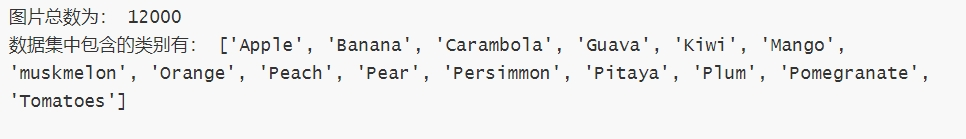
\includegraphics[width=\linewidth]{image/6/数据集输出1.png}}
  \caption{数据集概览输出图}
  \label{数据集概览输出图}
\end{figure}

从输出结果可以了解到，我们所使用的数据集包含12000张图片，分为15个不同的类别，每个类别代表一种水果。具体来说，数据集中包含以下水果类别：
\begin{multicols}{3} % 设置三列布局
\begin{itemize}
  \item Apple
  \item Banana
  \item Carambola
  \item Guava
  \item Kiwi
  \item Mango
  \item Muskmelon
  \item Orange
  \item Peach
  \item Pear
  \item Persimmon
  \item Pitaya
  \item Plum
  \item Pomegranate
  \item Tomatoes
\end{itemize}
\end{multicols}
我们想进一步探寻文件的结构，代码如Listing \ref{随机查看}所示。
\begin{lstlisting}[language={python},label={随机查看},caption={随机查看}, basicstyle=\footnotesize\ttfamily, breaklines=true, numbers=left, frame=single]
# 随机查看每个类别中的几张图片及其路径
for category in categories:
    category_dir = data_dir / category
    sample_images = list(category_dir.glob('*'))[:3]  # 每个类别查看3张图片
    print(f"\n类别 '{category}' 中的示例图片路径：")
    for image_path in sample_images:
        print(image_path)
\end{lstlisting}

输出如图\ref{数据集随机查看输出图}所示。
\begin{figure}[H]
  \centering
  \fbox{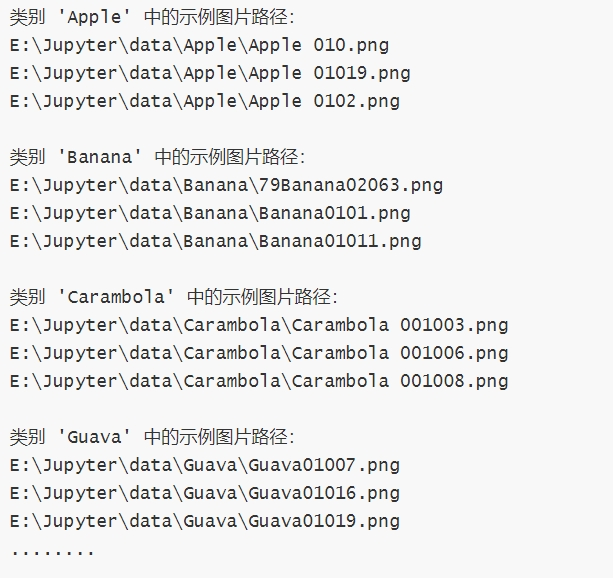
\includegraphics[width=10cm]{image/6/数据集输出2.png}}
  \caption{数据集随机查看输出图}
  \label{数据集随机查看输出图}
\end{figure}

图片尺寸很重要，关系到后续模型的输入格式、训练效率以及最终的预测效果。如果图片尺寸不统一，可能会导致模型无法正常训练或性能下降，我们通过代码Listing \ref{图片尺寸}来查看图片尺寸情况。
\begin{lstlisting}[language={python},label={图片尺寸},caption={图片尺寸}, basicstyle=\footnotesize\ttfamily, breaklines=true, numbers=left, frame=single]
# 检查所有图片的尺寸
image_sizes = {}
for image_path in data_dir.glob('*/*'):  # 遍历所有图片
    with Image.open(image_path) as img:
        size = img.size  # 获取图片尺寸 (width, height)
        if size not in image_sizes:
            image_sizes[size] = []  # 初始化该尺寸的图片列表
        image_sizes[size].append(image_path)

# 输出不同的图片尺寸及其对应的数量
print("\n图片尺寸统计：")
for size, paths in image_sizes.items():
    print(f"尺寸 {size} 的图片数量: {len(paths)}")

# 如果有多种尺寸，列出样例图片路径
if len(image_sizes) > 1:
    print("\n不同尺寸的样例图片：")
    for size, paths in image_sizes.items():
        print(f"\n尺寸 {size} 的部分图片：")
        for path in paths[:3]:  # 每种尺寸列出3个示例图片路径
            print(path)
else:
    print("\n所有图片的尺寸一致。")
\end{lstlisting}

输出如图\ref{图片尺寸输出图}所示。
数据集中的图片具有不同的尺寸，主要分为两种尺寸：
\begin{enumerate}
    \item 尺寸 (480, 322) 的图片，共有1339张
    \item 尺寸 (320, 258) 的图片，共有10661张。
\end{enumerate}
并且同一类别的图片也存在大小不统一的情况。

这种尺寸差异可能是由于拍摄设备或图像采集条件不同所导致的。为了确保后续训练过程中图像的统一性，我们将在数据预处理阶段通过代码Listing \ref{数据预处理}对图像尺寸进行调整。
\begin{figure}[ht]
  \centering
  \fbox{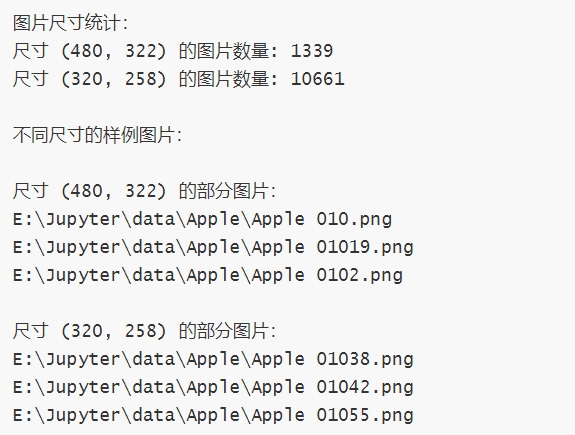
\includegraphics[width=10cm]{image/6/数据集输出3.png}}
  \caption{图片尺寸输出图}
  \label{图片尺寸输出图}
\end{figure}
我们通过以上步骤查看了数据集大小、图片路径与尺寸大小，更好地了解数据集的构成，这对后续的数据预处理和模型设计至关重要。

\subsection{数据划分与批处理}

数据划分是机器学习中的一个重要步骤，它决定了模型训练的效果和泛化能力。通常情况下，我们会将数据集分为训练集、验证集和测试集：
\begin{itemize}
    \item \textbf{训练集（Training Set）}：用于训练模型，包含大量的标注数据。模型通过这些数据来学习图像与标签之间的关系。
    \item \textbf{验证集（Validation Set）}：用于调整模型参数，验证模型在训练过程中是否有过拟合或欠拟合现象。验证集不参与训练，但用于中途的调优过程。
    \item \textbf{测试集（Test Set）}：用于评估最终训练完成的模型的性能。测试集只用于模型的最后评估，不参与任何训练过程。
\end{itemize}

这种划分的主要目的是通过训练集和验证集的反复调整，提升模型的泛化能力，避免模型在仅有的训练数据上过拟合，从而确保在新的数据上仍能保持良好的表现。

在数据划分后，我们还需要对数据进行批处理（batching）。批处理的意义在于，深度学习模型通常需要在大量数据上进行训练。如果每次训练时都加载所有数据，会消耗大量内存资源，甚至导致内存溢出。为了避免这一问题，我们将数据划分为多个小批次（batch），每次训练时仅加载一个批次的数据进行计算，这样能够显著提高训练效率，同时也能减少内存的消耗。

接下来，我们将使用Listing \ref{数据划分与批处理}代码来加载和划分数据集，并进行批处理：
\begin{lstlisting}[language={python},label={数据划分与批处理},caption={数据划分与批处理}, basicstyle=\footnotesize\ttfamily, breaklines=true, numbers=left, frame=single]
batch_size = 16

train_ds_raw = tf.keras.preprocessing.image_dataset_from_directory(
    data_dir,
    validation_split=0.2,
    subset="training",
    seed=12,
    batch_size=batch_size,
    follow_links=True)

val_ds_raw = tf.keras.preprocessing.image_dataset_from_directory(
    data_dir,
    validation_split=0.2,
    subset="validation",
    seed=12,
    batch_size=batch_size,
    follow_links=True)
\end{lstlisting}

划分结果如图\ref{数据集划分}所示，我们已经找到了包含15个类总共12000个文件，其中9600个文件中的数据被用作训练，剩下2400个文件中的数据被用于验证。让我们回到代码部分，来看看各部分发挥的作用，这段代码通过 \texttt{image\_dataset\_from\_directory} 函数（来自 \texttt{tf.keras.preprocessing} 模块）从指定的目录中加载图像数据，并将数据集划分为训练集和验证集：
\begin{figure}[ht]
  \centering
  \fbox{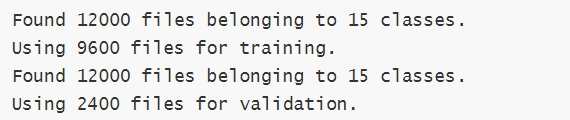
\includegraphics[width=10cm]{image/6/数据集划分.png}}
  \caption{数据集划分输出图}
  \label{数据集划分}
\end{figure}

\begin{itemize}
    \item \textbf{train\_ds\_raw}：训练集数据，包含数据目录中的 80\% 图像。通过$'validation\_split=0.2'$和$'subset=``training"'$选项指定。
    \item \textbf{val\_ds\_raw}：验证集数据，包含数据目录中的 20\% 图像。通过$'validation\_split=0.2'$和$'subset=``validation"'$选项指定。
    \item \textbf{batch\_size}：每次训练时加载的批次大小，这里设置为 16。每个批次包含 16 张图像。
    \item \textbf{follow\_links}：指定是否跟随符号链接加载数据。
    \item \textbf{seed}：随机种子，保证每次划分的数据集相同，确保结果的可复现性。
\end{itemize}

通过这种数据加载方式，我们可以方便地进行训练和验证，并控制批次的大小来提高训练效率。

\subsection{数据预处理}
\label{数据预处理}
数据预处理是机器学习中的关键步骤，它包括对图像的各种调整与优化操作，以保证训练的高效性与稳定性。常见的预处理步骤包括：

\begin{itemize}
    \item \textbf{统一图像大小}：深度学习模型对输入数据的尺寸有严格要求，因此我们通常会将所有图像统一调整为固定尺寸。例如，可以将图像缩放为$224 \times 224$像素。这样，模型能够在每次输入时处理一致的输入尺寸。
    \item \textbf{归一化像素值}：原始图像的像素值通常在$0-255$的范围内，而神经网络通常在$0-1$的浮动范围内效果更好。因此，我们需要将像素值缩放到0到1之间，通常的做法是将像素值除以255。
    \item \textbf{数据增强（Data Augmentation）}：为了提高模型的泛化能力，可以对图像进行各种变化，例如随机旋转、裁剪、翻转、改变亮度等。数据增强能够帮助模型更好地适应不同的输入，防止过拟合。
    \item \textbf{数据预取与缓存}：数据预取和缓存技术可以大幅提高训练速度。通过预取和缓存机制，我们可以在训练时提前加载数据并存储到内存中，避免每次训练时都从磁盘读取数据，减少I/O操作带来的延迟。
\end{itemize}

我们将跟随Listing \ref{数据预处理}代码部分，进行预处理操作：

\begin{lstlisting}[language={python},label={数据预处理},caption={数据预处理}, basicstyle=\footnotesize\ttfamily, breaklines=true, numbers=left, frame=single]
AUTOTUNE = tf.data.AUTOTUNE

def train_preprocessing(image, label):
    image = tf.image.random_flip_left_right(image)  # 随机水平翻转
    image = tf.image.random_brightness(image, 0.2)  # 随机亮度
    #image = tf.image.random_zoom(image, (0.9, 1.1)) # 随机缩放
    image = tf.image.resize(image, [224, 224])
    return (image / 255.0, label)  #归一化

def val_preprocessing(image, label):
    image = tf.image.resize(image, [224, 224])
    image = image / 255.0  # 归一化到 [0, 1]
    return image, label

# 然后再进行数据预处理
train_ds = train_ds_raw.map(train_preprocessing).cache().shuffle(1000).prefetch(buffer_size=AUTOTUNE) #shuffle()：打乱数据集
val_ds = val_ds_raw.cache().map(val_preprocessing).prefetch(buffer_size=AUTOTUNE)# 获取类别名称
class_names = train_ds_raw.class_names
print("数据类别有：", class_names)
print("识别的水果一共%d类" % len(class_names))


AUTOTUNE = tf.data.AUTOTUNE

def train_preprocessing(image, label):
    image = tf.image.resize(image, [224, 224]) #resize图片大小
    return (image / 255.0, label)  #归一化

# 然后再进行数据预处理
train_ds = train_ds_raw.cache().map(train_preprocessing).prefetch(buffer_size=AUTOTUNE)
val_ds = val_ds_raw.cache().map(train_preprocessing).prefetch(buffer_size=AUTOTUNE)
\end{lstlisting}

该代码片段首先加载图像数据，并对训练集和验证集进行预处理操作，包括数据增强、图像大小调整、像素值归一化和缓存与预取：
\begin{itemize}
     \item \textbf{数据增强}：在训练数据预处理函数 $train\_preprocessing$ 中，使用了两个数据增强操作：随机水平翻转和随机亮度变化。这些操作可以增加数据的多样性，从而提高模型的泛化能力。
    \item \textbf{图像调整大小}：在训练和验证数据的预处理函数中，都使用了 $'tf.image.resize'$ 对图像进行大小调整，将所有图像的尺寸调整为 $224 \times 224$，这是一个常见的输入尺寸。
    \item \textbf{归一化}：归一化操作通过将图像像素值从 $0-255$ 范围转换到 $0-1$，帮助模型更容易训练。
    \item \textbf{缓存和预取}：为了提高训练效率，代码使用了 $'cache'$ 和 $'prefetch'$ 操作。$'cache'$ 会将数据集缓存到内存中，避免每次读取数据时都需要访问磁盘。$'prefetch'$ 会提前加载数据，以减少训练过程中由于 I/O 操作带来的延迟。
\end{itemize}
注意，尤其是在大规模数据集的情况下，这些操作将有助于提高模型的性能和训练效率。
而完成数据预处理后，我们通常希望对处理后的图像进行可视化展示。这样做不仅能帮助我们验证预处理的效果，还能直观地看到图像在经过预处理后的变化，例如是否存在扭曲或颜色失真等问题。实现方法如所示：
\begin{lstlisting}[language={python},label={数据预处理},caption={数据预处理}, basicstyle=\footnotesize\ttfamily, breaklines=true, numbers=left, frame=single]
# 可视化数据
plt.figure(figsize=(10, 8))  # 图形的宽为10高为8
plt.suptitle("数据展示")

# 只取一批次的数据来进行展示
for images, labels in train_ds.take(1):
    for i in range(15):
        plt.subplot(4, 5, i + 1)
        plt.xticks([])
        plt.yticks([])
        plt.grid(False)

        # 显示图片
        plt.imshow(images[i])
        # 显示标签
        plt.xlabel(class_names[labels[i]])

plt.show()
\end{lstlisting}
输出结果如图\ref{预处理图像展示}所示。可以看到，展示部分的图像大小是统一的。
\begin{figure}[ht]
  \centering
  \fbox{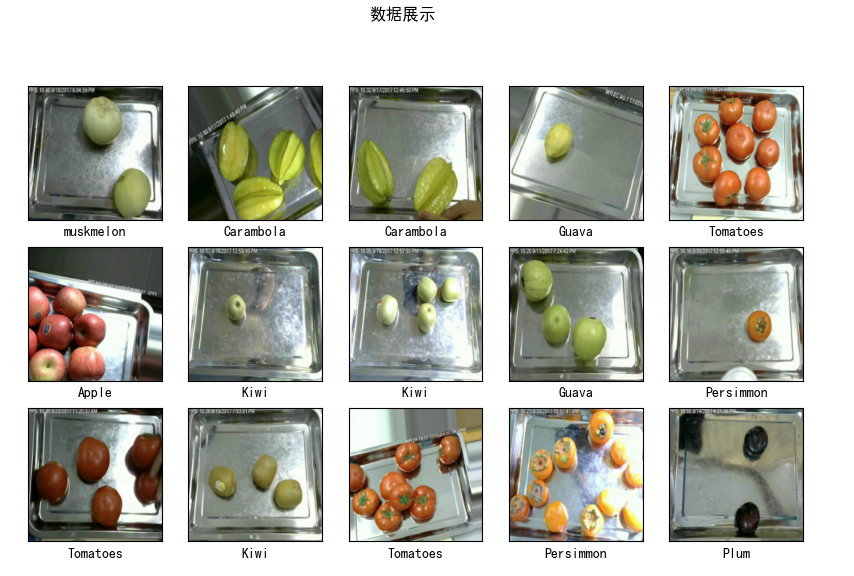
\includegraphics[width=\linewidth]{image/6/预处理图像展示.png}} % 添加黑框
  \caption{数据可视化展示}
  \label{预处理图像展示}
\end{figure}

\section{深度学习模型构建}
在数据预处理工作完成后，我们将进入模型构建阶段。这里，我们将通过搭建深度学习模型来完成水果图像分类的任务。在这个过程中，构建模型的架构是至关重要的一步，它决定了模型的学习能力和性能。
深度学习模型的训练通常需要大量的计算资源和时间。而在实际应用中，我们并不总是需要从零开始训练一个全新的模型。为了减少训练时间和成本，我们可以利用“迁移学习”策略，加载预先训练好的模型（即预训练模型）。

我们将使用 \textbf{ResNet50} 模型，ResNet50是一个深度卷积神经网络，已经在大规模图像数据集上进行了训练，具备较强的特征提取能力。通过加载这个模型的预训练权重，我们可以避免从头开始训练一个深度网络，并且直接获得一个较好的特征提取器。

通过这种方式，我们不仅能够缩短训练时间，还能提升模型的表现。预训练模型提供了一个强大的起点，使我们可以在已有的基础上进行微调，以适应我们的水果分类任务。

\subsection{添加自定义层}

尽管ResNet50模型已经可以处理大量图像分类任务，但它的原始结构是针对ImageNet数据集进行训练的，包含了1000个类别。而我们的水果分类任务只有少数几类水果，因此需要对模型进行调整，以便更好地适应我们的数据。

在预训练模型的基础上，我们通过添加自定义层，来调整模型的输出层，以适应我们的任务，代码如Listing \ref{添加自定义层}所示。
\begin{lstlisting}[language={python},label={添加自定义层},caption={添加自定义层}, basicstyle=\footnotesize\ttfamily, breaklines=true, numbers=left, frame=single]
X = base_model.output
X = Flatten()(X)
X = Dense(512, kernel_initializer='he_uniform')(X)
X = BatchNormalization()(X)
X = Activation('relu')(X)
X = Dense(15, kernel_initializer='he_uniform')(X)
X = BatchNormalization()(X)
X = Activation('relu')(X)
output = Dense(len(class_names), activation='softmax')(X)

model = Model(inputs=base_model.input, outputs=output)
\end{lstlisting}

首先，我们提取了预训练模型的输出（\texttt{base\_model.output}），并通过 \texttt{Flatten()} 将其转换为一维向量，方便后续处理。接着，我们添加了一层全连接层（\texttt{Dense(512)})，这一层有 512 个神经元，用来提取更高层次的特征。这里使用了批量归一化（\texttt{BatchNormalization()}）来提高训练的稳定性，同时使用激活函数 \texttt{ReLU} 增强模型的非线性表现能力。

随后，我们添加了另一层全连接层（\texttt{Dense(15)}），这一层的神经元数量设置为 15，是因为我们任务中有 15 种水果类别。这样可以进一步压缩特征，并使模型更聚焦于我们关心的分类目标。

最后，我们定义了输出层（\texttt{Dense(len(class\_names), activation='softmax')}），这一层的神经元数量与我们数据集中的水果类别数一致（15），通过 \texttt{softmax} 激活函数将结果转换为每种水果类别的概率分布，用于最终分类。

通过这些调整，我们的模型在保留ResNet50原有特征提取能力的基础上，针对水果分类任务进行了定制化设计，从而能够更准确地完成分类任务。

\section{正式开始训练模型}

本部分介绍从已有的模型结构出发，开始实际训练的过程，让读者了解训练时涉及的关键步骤和思考角度。

\subsection{编译模型}

编译模型是深度学习训练中的一个重要步骤，它相当于为模型设定了学习的策略和目标。在这一阶段，我们需要选择优化器、损失函数和评价指标等元素，这些将直接影响到模型的训练行为。

\begin{itemize}
    \item \textbf{优化器（Optimizer）}：优化器决定了模型如何更新参数。常见的优化器有Adam、SGD（随机梯度下降）等。选择优化器时，我们需要根据任务和数据的特点来做出决定。优化器的选择会直接影响模型训练的速度和最终的效果。
    \item \textbf{损失函数（Loss Function）}：损失函数用于衡量模型预测值与实际值之间的差异。在图像分类任务中，常用的损失函数是交叉熵损失函数（Cross-Entropy Loss）。损失函数的选择关系到模型训练的方向，它告诉模型在每次迭代时应该如何调整参数。
    \item \textbf{评价指标（Metrics）}：评价指标用于评估模型在训练过程中的表现。常见的指标包括准确率（Accuracy）、精确率（Precision）、召回率（Recall）等。在训练过程中，我们通过这些指标来观察模型的进展。
\end{itemize}
对于本任务，我们选择了Adam优化器、交叉熵损失函数以及准确率作为评估指标，代码如Listing \ref{编译模型}所示。
\begin{lstlisting}[language={python},label={编译模型},caption={编译模型}, basicstyle=\footnotesize\ttfamily, breaklines=true, numbers=left, frame=single]
optimizer = tf.keras.optimizers.Adam(learning_rate=1e-5)

model.compile(optimizer=optimizer,
              loss='sparse_categorical_crossentropy',
              metrics=['accuracy'])
\end{lstlisting}
\subsection{设置回调函数}

在训练过程中，我们往往需要一些机制来动态地调整训练的过程，以提升训练效率和模型的性能。回调函数（Callbacks）便是实现这一目标的工具。

回调函数可以帮助我们在训练过程中自动执行某些操作，例如：
\begin{itemize}
    \item \textbf{早停（Early Stopping）}：当模型在验证集上的表现不再提升时，自动停止训练，以防止过拟合。
    \item \textbf{学习率调整（Learning Rate Scheduling）}：根据训练的进展动态调整学习率，帮助模型在不同阶段以最优速度收敛。
    \item \textbf{模型保存（Model Checkpoints）}：定期保存当前最优模型，以防止训练过程中断时丢失进度。
\end{itemize}
通过执行以上操作，我们能确保在验证集最优时保存模型，实现代码如Listing \ref{设置回调函数}所示。
\begin{lstlisting}[language={python},label={设置回调函数},caption={设置回调函数}, basicstyle=\footnotesize\ttfamily, breaklines=true, numbers=left, frame=single] 
from tensorflow.keras.callbacks import ModelCheckpoint, Callback, EarlyStopping, ReduceLROnPlateau, LearningRateScheduler

NO_EPOCHS = 10
PATIENCE  = 5
VERBOSE   = 1

# 设置早停
earlystopper = EarlyStopping(monitor='loss', patience=PATIENCE, verbose=VERBOSE)
checkpointer = ModelCheckpoint('best_model.weights.h5', 
                                monitor='val_accuracy', 
                                verbose=VERBOSE, 
                                save_best_only=True, 
                                save_weights_only=True)

\end{lstlisting}

这些回调机制不仅能提升训练效率，还能确保训练过程的稳定性和模型的性能。注意，读者需要理解回调机制的意义，而不是关注每种回调的具体实现细节。通过这些回调，训练过程能够更加智能化和高效。

\subsection{训练模型}

模型编译和回调函数设置完毕后，我们可以开始实际的训练过程。在训练时，模型会通过多次迭代（Epoch）逐步调整参数，以优化其性能。
在每一次训练迭代中，模型会根据当前的参数和输入数据，计算损失并通过反向传播算法更新参数。训练的核心逻辑可以总结为：
\begin{itemize}
    \item \textbf{逐步更新参数}：每次迭代后，模型的参数（如权重和偏置）都会根据损失函数的梯度更新，从而使模型的预测值逐步接近真实标签。
    \item \textbf{迭代次数（Epochs）}：训练通常需要多个迭代周期（Epochs）。每一个周期代表模型遍历整个训练集一次。一般来说，较多的迭代周期有助于提高模型的准确性，但过多的迭代可能会导致过拟合。
    \item \textbf{模型性能提升的期望}：随着训练的进行，模型的损失函数值应逐渐下降，准确率应逐渐上升。理想情况下，模型在训练集和验证集上的表现都应有所提升。
\end{itemize}

训练的实现代码如Listing \ref{模型训练代码} 所示：

\begin{lstlisting}[language=python, label={模型训练代码}, caption={模型训练过程}, basicstyle=\footnotesize\ttfamily, breaklines=true, numbers=left, frame=single]
train_model = model.fit(train_ds,
                        epochs=NO_EPOCHS,
                        verbose=VERBOSE,
                        validation_data=val_ds,
                        callbacks=[earlystopper, checkpointer])
\end{lstlisting}

在这段代码中：
\begin{itemize}
    \item \texttt{train\_ds} 和 \texttt{val\_ds} 分别是训练数据集和验证数据集，用于模型在每次迭代中学习和验证性能。
    \item \texttt{epochs=NO\_EPOCHS} 指定了训练的迭代次数（在Listing \ref{设置回调函数}中，我们定义好了NO\_EPOCHS = 10），即模型会完整遍历训练集的次数为10次。
    \item \texttt{verbose=VERBOSE} 控制训练过程的日志输出级别，例如显示每次迭代的损失和准确率。
    \item \texttt{validation\_data=val\_ds} 表明在每个训练周期结束后，模型会在验证集上进行评估，帮助监控模型在验证数据上的表现。
    \item \texttt{callbacks=[earlystopper, checkpointer]} 是在回调函数中使用Listing \ref{设置回调函数}的早停设置。
\end{itemize}

通过我们的日志输出级别控制，能看到运行结果如图\ref{迭代日志信息}所示。
\begin{figure}[ht]
  \centering
  \fbox{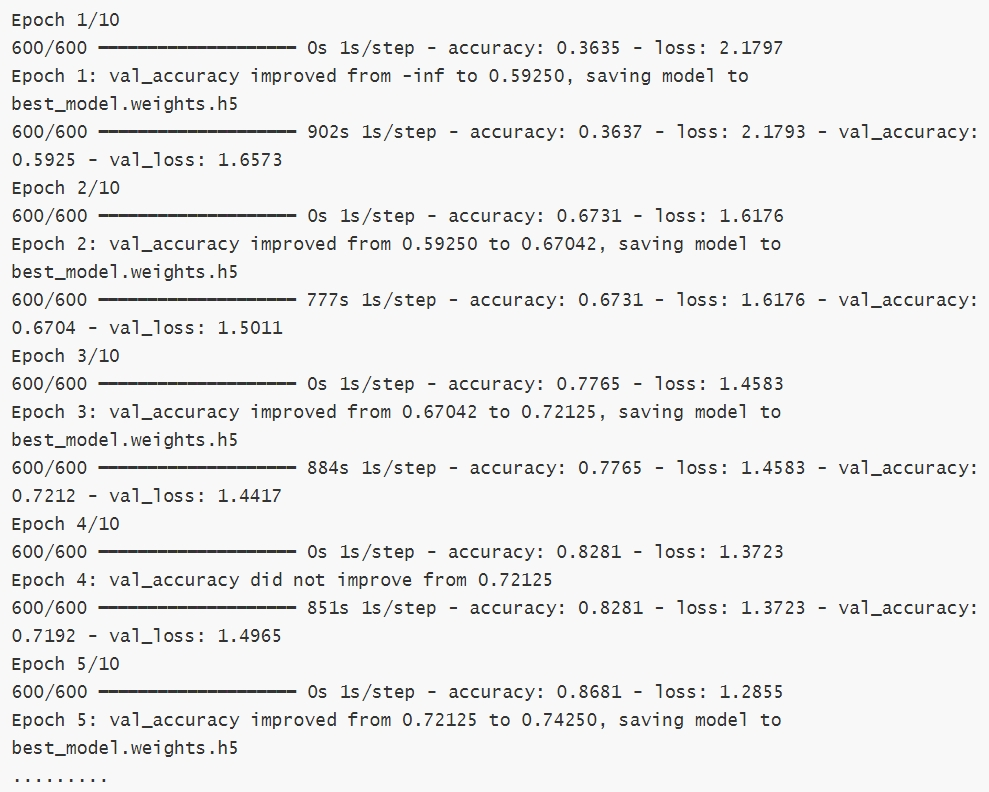
\includegraphics[width=\linewidth]{image/6/迭代日志信息.png}}
  \caption{迭代日志信息}
  \label{迭代日志信息}
\end{figure}

读者也可以改变我们的迭代次数，去看看不同的训练效果吧！训练过程是一个不断试错和优化的过程。通过调节参数和调整训练策略，我们最终能够得到一个性能良好的模型。训练过程中需要注意观察模型的各项指标，以确保模型在学习的过程中稳定收敛。

\section{测试我们的模型}

在模型训练完成后，接下来就是评估其性能的阶段。测试阶段通过验证和评价手段，让读者直观感受到模型在实际任务上的表现。评价阶段为整个项目提供闭环，让前面所有环节的效果有据可查。

\subsection{可视化训练过程}

在训练完成后，我们通常会通过可视化手段，回顾模型在训练和验证过程中的表现。具体来说，我们会绘制损失和准确率随时间变化的曲线，帮助我们分析训练过程中的动态变化。

\begin{itemize}
    \item \textbf{训练曲线和验证曲线}：我们可以绘制训练损失、验证损失、训练准确率和验证准确率的变化曲线。通过观察这些曲线，我们可以判断模型是否过拟合或欠拟合。如果训练准确率持续提升而验证准确率停滞不前，可能意味着过拟合；反之，如果两者的准确率都较低，则可能是欠拟合。
    \item \textbf{训练过程的评估}：通过训练曲线，我们可以清晰地看到模型是否达到理想状态。例如，损失函数趋于平稳，准确率稳定在较高水平时，模型通常意味着训练已经完成，且性能已趋于最优。
\end{itemize}

我们的实现代码如Listing \ref{准确率及损失曲线}所示。
\begin{lstlisting}[language=python, label={准确率及损失曲线}, caption={准确率及损失曲线}, basicstyle=\footnotesize\ttfamily, breaklines=true, numbers=left, frame=single]
acc = train_model.history['accuracy']
val_acc = train_model.history['val_accuracy']

loss = train_model.history['loss']
val_loss = train_model.history['val_loss']

epochs_range = range(len(acc))

plt.figure(figsize=(12, 4))
plt.subplot(1, 2, 1)
plt.plot(epochs_range, acc, label='Training Accuracy')
plt.plot(epochs_range, val_acc, label='Validation Accuracy')
plt.legend(loc='lower right')
plt.title('Training and Validation Accuracy')

plt.subplot(1, 2, 2)
plt.plot(epochs_range, loss, label='Training Loss')
plt.plot(epochs_range, val_loss, label='Validation Loss')
plt.legend(loc='upper right')
plt.title('Training and Validation Loss')
plt.show()
\end{lstlisting}
通过执行以上代码，我们能得到如图\ref{准确率及损失曲线图}的结果。
\begin{figure}[ht]
  \centering
  \fbox{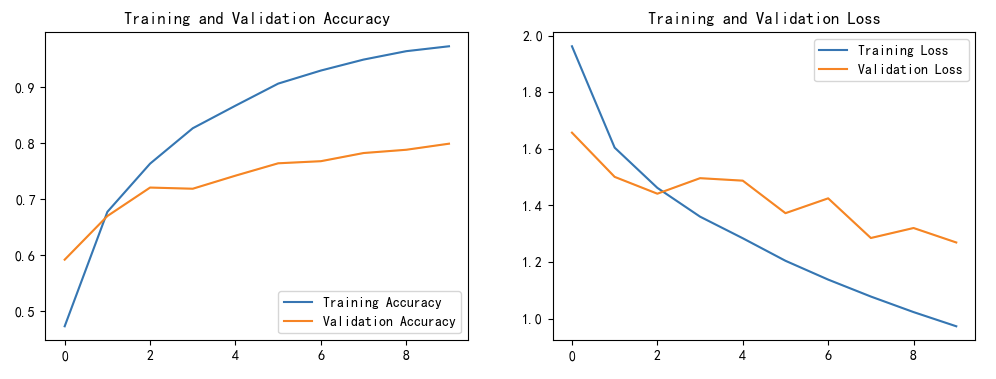
\includegraphics[width=\linewidth]{image/6/epoch可视化.png}}
  \caption{准确率及损失曲线图}
  \label{准确率及损失曲线图}
\end{figure}


左图展示了训练和验证的准确率随迭代次数的变化。可以观察到，训练准确率随着迭代次数的增加逐渐提升，并最终接近 1.0，这表明模型在训练集上表现良好。然而，验证集的准确率相对较低，且在训练后期趋于平稳，未能达到训练集的水平。这可能表明模型在验证集上的泛化能力有限。

右图展示了训练和验证的损失值随迭代次数的变化。训练损失值持续下降，表明模型在训练集上不断学习并优化。然而，验证损失值虽然整体下降，但在训练后期波动较大，可能反映出模型在验证集上的拟合能力不够稳定。

通过这些曲线，可以得出以下结论：
\begin{itemize}
    \item \textbf{训练准确率较高，验证准确率较低}：训练集和验证集的准确率差距较大，表明模型可能存在一定程度的过拟合，即模型在训练集上表现很好，但在验证集上表现不佳。
    \item \textbf{验证损失值波动}：验证损失值的波动可能说明模型对验证数据的适应性不足，可能需要更好的正则化方法或更多的验证数据来提升泛化性能。
    \item \textbf{改进方向}：可以通过增加数据集的多样性、调整模型结构或优化超参数（如学习率、批量大小）来提升验证集的表现。
\end{itemize}

总体来说，模型在训练集上的性能优异，但在验证集上的表现有限。这些现象需要进一步的优化和调整，以提高模型的泛化能力，确保其在实际应用场景中的可靠性。
\subsection{混淆矩阵}

混淆矩阵是评估分类模型性能的一个重要工具。它可以帮助我们了解模型在不同类别上的识别能力，以及哪些类别容易混淆。

\begin{itemize}
    \item \textbf{分析模型的误差}：混淆矩阵展示了每个类别预测的情况，其中包括正确分类和错误分类的数量。通过查看哪些类别容易被混淆，读者可以进一步优化数据集或调整模型，以提高对这些类别的识别能力。
    \item \textbf{深入探索模型性能}：混淆矩阵不仅可以帮助我们看到整体的分类准确率，还可以揭示哪些类别更容易被误分类。理解这些误差对于模型的进一步优化至关重要。
\end{itemize}
我们的实现代码如Listing \ref{混淆矩阵代码}所示。
\begin{lstlisting}[language=python, label={混淆矩阵代码}, caption={混淆矩阵代码}, basicstyle=\footnotesize\ttfamily, breaklines=true, numbers=left, frame=single]
from sklearn.metrics import confusion_matrix
import seaborn as sns
import pandas as pd

def plot_cm(labels, predictions):
    conf_numpy = confusion_matrix(labels, predictions)
    conf_df = pd.DataFrame(conf_numpy, index=class_names, columns=class_names)
    plt.figure(figsize=(8, 7))
    sns.heatmap(conf_df, annot=True, fmt="d", cmap="BuPu")
    plt.title('混淆矩阵', fontsize=15)
    plt.ylabel('真实值', fontsize=14)
    plt.xlabel('预测值', fontsize=14)
    
val_pre   = []
val_label = []

for images, labels in val_ds:#这里可以取部分验证数据（.take(1)）生成混淆矩阵
    for image, label in zip(images, labels):
        # 需要给图片增加一个维度
        img_array = tf.expand_dims(image, 0) 
        # 使用模型预测图片中的人物
        prediction = model.predict(img_array)

        val_pre.append(class_names[np.argmax(prediction)])
        val_label.append(class_names[label])
 plot_cm(val_label, val_pre)
\end{lstlisting}

通过执行以上代码，我们能得到如图\ref{混淆矩阵}的结果。其纵轴为真实标签，横轴为模型预测标签。对角线上的数字表示模型将样本正确分类的数量，颜色越深表示分类正确的数量越多。例如，`Apple` 被正确分类了 84 次，`Carambola` 被正确分类了 153 次，`Persimmon` 被正确分类了 176 次。这表明模型对这些类别的分类效果较好。

然而，非对角线上的数字表示分类错误的样本数量，反映了类别间的混淆情况。例如：
\begin{itemize}
    \item $'Apple'$ 有 27 个样本被错误分类为$'Muskmelon'$，说明这两个类别之间存在较大的混淆。
    \item $'Kiwi'$ 和 $'Muskmelon'$ 之间也有较大的混淆，有 6 个样本被错误分类。
    \item 类似地，$'Guava'$ 和 $'Kiwi'$ 也存在一定程度的分类错误，反映模型对这两种类别的区分能力有限。
\end{itemize}

总的来看，模型对部分类别的分类效果较好，例如$'Carambola'$和$'Persimmon'$，这些类别的分类正确率较高。但对于某些类别，如 $'Apple'$ 和 $'Muskmelon'$，以及 $'Kiwi'$ 和 $'Guava'$，模型在区分它们时表现出一定的不足。

这些结果表明，模型在训练过程中能够有效地学习大部分类别的特征，但对于某些相似类别，还需要进一步优化以减少混淆。这可以通过增加数据集样本量、使用更复杂的模型结构或应用数据增强技术来改善。
\begin{figure}[ht]
  \centering
  \fbox{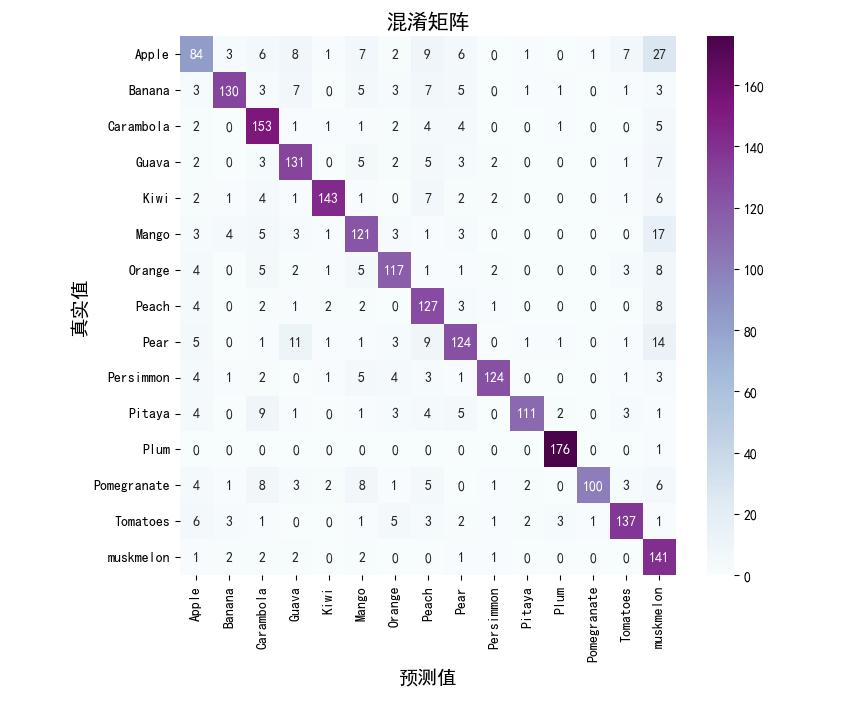
\includegraphics[width=\linewidth]{image/6/混淆矩阵.png}}
  \caption{混淆矩阵}
  \label{混淆矩阵}
\end{figure}
\subsection{模型评估报告}

在最后，我们将模型的评估结果以简洁明了的方式呈现，包括准确率、召回率、精确率、F1值等重要指标，这些指标提供了模型性能的全貌，使读者可以全面了解模型的优缺点：
\begin{itemize}
    \item \textbf{准确率（Accuracy）}：衡量模型正确分类的样本所占比例。
    \item \textbf{精确率（Precision）}：衡量模型正确预测为正类的样本占所有预测为正类的样本的比例。
    \item \textbf{召回率（Recall）}：衡量模型正确预测为正类的样本占所有实际为正类的样本的比例。
    \item \textbf{F1值}：精确率和召回率的调和平均值，综合了模型在精确度和召回率上的表现。
\end{itemize}
我们的实现代码如Listing \ref{评估报告代码}所示。
\begin{lstlisting}[language=python, label={评估报告代码}, caption={评估报告代码}, basicstyle=\footnotesize\ttfamily, breaklines=true, numbers=left, frame=single]
from sklearn import metrics

def test_accuracy_report(model):
    print(metrics.classification_report(val_label, val_pre, target_names=class_names)) 
    score = model.evaluate(val_ds, verbose=0)
    print('Loss function: %s, accuracy:' % score[0], score[1])

test_accuracy_report(model)
\end{lstlisting}
通过执行以上代码，我们能得到如图\ref{评估报告}的结果。
\begin{figure}[ht]
  \centering
  \fbox{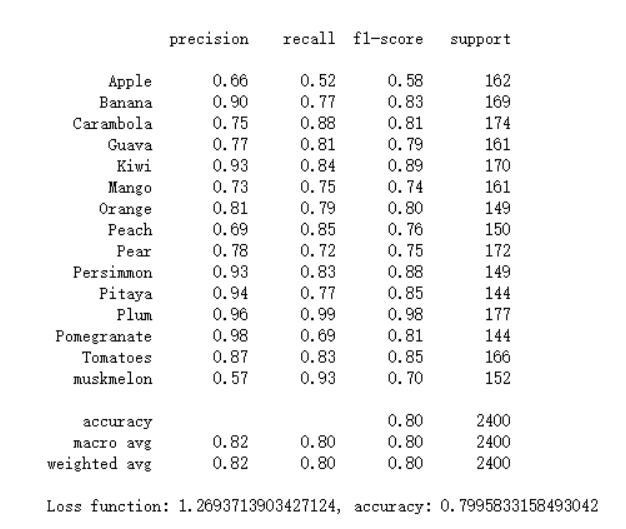
\includegraphics[width=\linewidth]{image/6/评估报告.png}}
  \caption{评估报告}
  \label{评估报告}
\end{figure}
根据报告，我们能作出以下分析：

\begin{itemize}
    \item \textbf{总体表现}：
        \begin{itemize}
            \item 模型在 2400 个测试样本上的平均准确率为 \textbf{80\%}。
            \item 宏平均（macro avg）和加权平均（weighted avg）的精确率（precision）、召回率（recall）和 F1 分数均接近 \textbf{80\%}，表明模型对不同类别的性能较为均衡。
        \end{itemize}

    \item \textbf{分类表现较好的类别}：
        \begin{itemize}
            \item $'Plum'$达到了最高的 F1 分数（\textbf{0.98}），表明其分类效果非常优异。
            \item $'Kiwi'$和$'Persimmon'$的 F1 分数也较高，分别为 \textbf{0.89} 和 \textbf{0.88}，表现稳定。
        \end{itemize}

    \item \textbf{分类存在挑战的类别}：
        \begin{itemize}
            \item $'Apple'$的召回率为 \textbf{0.52}，F1 分数为 \textbf{0.58}，表明模型对该类别的识别能力较弱。
            \item $'Muskmelon'$的精确率较低（\textbf{0.57}），但召回率较高（\textbf{0.93}），表明模型更倾向于预测该类别，从而导致一定的误分类。
            \item 类别$'Pomegranate'$的召回率仅为 \textbf{0.69}，表明模型对该类别的一部分样本未能正确分类。
        \end{itemize}
\end{itemize}
总体来看，模型能够较好地处理大部分类别的分类任务，但在某些类别上（如$'Apple'$ 和 $'Muskmelon'$）仍存在改进空间。

到此，我们的第一个人工智能项目就圆满完成啦，希望读者能跟随着我们的代码，动手实践出你自己的第一个人工智能项目！



